\documentclass[twoside]{book}

% Packages required by doxygen
\usepackage{fixltx2e}
\usepackage{calc}
\usepackage{doxygen}
\usepackage[export]{adjustbox} % also loads graphicx
\usepackage{graphicx}
\usepackage[utf8]{inputenc}
\usepackage{makeidx}
\usepackage{multicol}
\usepackage{multirow}
\PassOptionsToPackage{warn}{textcomp}
\usepackage{textcomp}
\usepackage[nointegrals]{wasysym}
\usepackage[table]{xcolor}

% Font selection
\usepackage[T1]{fontenc}
\usepackage[scaled=.90]{helvet}
\usepackage{courier}
\usepackage{amssymb}
\usepackage{sectsty}
\renewcommand{\familydefault}{\sfdefault}
\allsectionsfont{%
  \fontseries{bc}\selectfont%
  \color{darkgray}%
}
\renewcommand{\DoxyLabelFont}{%
  \fontseries{bc}\selectfont%
  \color{darkgray}%
}
\newcommand{\+}{\discretionary{\mbox{\scriptsize$\hookleftarrow$}}{}{}}

% Page & text layout
\usepackage{geometry}
\geometry{%
  a4paper,%
  top=2.5cm,%
  bottom=2.5cm,%
  left=2.5cm,%
  right=2.5cm%
}
\tolerance=750
\hfuzz=15pt
\hbadness=750
\setlength{\emergencystretch}{15pt}
\setlength{\parindent}{0cm}
\setlength{\parskip}{3ex plus 2ex minus 2ex}
\makeatletter
\renewcommand{\paragraph}{%
  \@startsection{paragraph}{4}{0ex}{-1.0ex}{1.0ex}{%
    \normalfont\normalsize\bfseries\SS@parafont%
  }%
}
\renewcommand{\subparagraph}{%
  \@startsection{subparagraph}{5}{0ex}{-1.0ex}{1.0ex}{%
    \normalfont\normalsize\bfseries\SS@subparafont%
  }%
}
\makeatother

% Headers & footers
\usepackage{fancyhdr}
\pagestyle{fancyplain}
\fancyhead[LE]{\fancyplain{}{\bfseries\thepage}}
\fancyhead[CE]{\fancyplain{}{}}
\fancyhead[RE]{\fancyplain{}{\bfseries\leftmark}}
\fancyhead[LO]{\fancyplain{}{\bfseries\rightmark}}
\fancyhead[CO]{\fancyplain{}{}}
\fancyhead[RO]{\fancyplain{}{\bfseries\thepage}}
\fancyfoot[LE]{\fancyplain{}{}}
\fancyfoot[CE]{\fancyplain{}{}}
\fancyfoot[RE]{\fancyplain{}{\bfseries\scriptsize Generated by Doxygen }}
\fancyfoot[LO]{\fancyplain{}{\bfseries\scriptsize Generated by Doxygen }}
\fancyfoot[CO]{\fancyplain{}{}}
\fancyfoot[RO]{\fancyplain{}{}}
\renewcommand{\footrulewidth}{0.4pt}
\renewcommand{\chaptermark}[1]{%
  \markboth{#1}{}%
}
\renewcommand{\sectionmark}[1]{%
  \markright{\thesection\ #1}%
}

% Indices & bibliography
\usepackage{natbib}
\usepackage[titles]{tocloft}
\setcounter{tocdepth}{3}
\setcounter{secnumdepth}{5}
\makeindex

% Hyperlinks (required, but should be loaded last)
\usepackage{ifpdf}
\ifpdf
  \usepackage[pdftex,pagebackref=true]{hyperref}
\else
  \usepackage[ps2pdf,pagebackref=true]{hyperref}
\fi
\hypersetup{%
  colorlinks=true,%
  linkcolor=blue,%
  citecolor=blue,%
  unicode%
}

% Custom commands
\newcommand{\clearemptydoublepage}{%
  \newpage{\pagestyle{empty}\cleardoublepage}%
}

\usepackage{caption}
\captionsetup{labelsep=space,justification=centering,font={bf},singlelinecheck=off,skip=4pt,position=top}

%===== C O N T E N T S =====

\begin{document}

% Titlepage & ToC
\hypersetup{pageanchor=false,
             bookmarksnumbered=true,
             pdfencoding=unicode
            }
\pagenumbering{roman}
\begin{titlepage}
\vspace*{7cm}
\begin{center}%
{\Large Socket\+Programming }\\
\vspace*{1cm}
{\large Generated by Doxygen 1.8.11}\\
\end{center}
\end{titlepage}
\clearemptydoublepage
\tableofcontents
\clearemptydoublepage
\pagenumbering{arabic}
\hypersetup{pageanchor=true}

%--- Begin generated contents ---
\chapter{Socket Programming}
\label{md_README}
\hypertarget{md_README}{}

\begin{DoxyItemize}
\item This is the \hyperlink{classSocket}{Socket} programming library in C++ for {\bfseries Linux} based systems.
\item It provides the interfaces defined in the respective header files {\ttfamily .h files}, with the implementation included in the {\ttfamily .cpp files} resp.
\item It explicitly defines the {\bfseries \hyperlink{classSocketClient}{Socket\+Client}} and {\bfseries \hyperlink{classSocketServer}{Socket\+Server}} library, both of which inherits the {\bfseries \hyperlink{classSocket}{Socket}} library which contains some of the coon functionalities.
\item Uses doxygen for documentation.
\end{DoxyItemize}

\tabulinesep=1mm
\begin{longtabu} spread 0pt [c]{*3{|X[-1]}|}
\hline
\rowcolor{\tableheadbgcolor}{\bf S.\+No$<$th$>$ File\+Name }&\PBS\centering {\bf Content  }\\\cline{1-3}
\endfirsthead
\hline
\endfoot
\hline
\rowcolor{\tableheadbgcolor}{\bf S.\+No$<$th$>$ File\+Name }&\PBS\centering {\bf Content  }\\\cline{1-3}
\endhead
1. &\hyperlink{Socket_8h}{Socket.\+h} &\PBS\centering Header file for generic \hyperlink{classSocket}{Socket} functionalities. \\\cline{1-3}
2. &\hyperlink{SocketClient_8h}{Socket\+Client.\+h} &\PBS\centering Header file for Socket-\/\+Client functionalities. \\\cline{1-3}
3. &\hyperlink{SocketServer_8h}{Socket\+Server.\+h} &\PBS\centering Header file for Socket-\/\+Server functionalities. \\\cline{1-3}
\end{longtabu}

\chapter{Hierarchical Index}
\section{Class Hierarchy}
This inheritance list is sorted roughly, but not completely, alphabetically\+:\begin{DoxyCompactList}
\item \contentsline{section}{Socket}{\pageref{classSocket}}{}
\begin{DoxyCompactList}
\item \contentsline{section}{Socket\+Client}{\pageref{classSocketClient}}{}
\item \contentsline{section}{Socket\+Server}{\pageref{classSocketServer}}{}
\end{DoxyCompactList}
\end{DoxyCompactList}

\chapter{Class Index}
\section{Class List}
Here are the classes, structs, unions and interfaces with brief descriptions\+:\begin{DoxyCompactList}
\item\contentsline{section}{\hyperlink{classSocket}{Socket} \\*Class responsible for managin low-\/level sockets }{\pageref{classSocket}}{}
\item\contentsline{section}{\hyperlink{classSocketClient}{Socket\+Client} \\*\textquotesingle{}\hyperlink{classSocketClient}{Socket\+Client}\textquotesingle{} inherits form \textquotesingle{}\hyperlink{classSocket}{Socket}\textquotesingle{} class and is specifically designed for client mode }{\pageref{classSocketClient}}{}
\item\contentsline{section}{\hyperlink{classSocketServer}{Socket\+Server} \\*\textquotesingle{}\hyperlink{classSocketServer}{Socket\+Server}\textquotesingle{} inherits form \textquotesingle{}\hyperlink{classSocket}{Socket}\textquotesingle{} class and is specifically designed for server mode }{\pageref{classSocketServer}}{}
\end{DoxyCompactList}

\chapter{File Index}
\section{File List}
Here is a list of all documented files with brief descriptions\+:\begin{DoxyCompactList}
\item\contentsline{section}{\hyperlink{Socket_8h}{Socket.\+h} \\*This file contains the \textquotesingle{}\hyperlink{classSocket}{Socket}\textquotesingle{} class }{\pageref{Socket_8h}}{}
\item\contentsline{section}{\hyperlink{SocketClient_8h}{Socket\+Client.\+h} \\*This file contains the \textquotesingle{}\hyperlink{classSocketClient}{Socket\+Client}\textquotesingle{} class }{\pageref{SocketClient_8h}}{}
\item\contentsline{section}{\hyperlink{SocketServer_8h}{Socket\+Server.\+h} \\*This file contains the \textquotesingle{}\hyperlink{classSocketServer}{Socket\+Server}\textquotesingle{} class }{\pageref{SocketServer_8h}}{}
\end{DoxyCompactList}

\chapter{Class Documentation}
\hypertarget{classSocket}{}\section{Socket Class Reference}
\label{classSocket}\index{Socket@{Socket}}


Class responsible for managin low-\/level sockets.  




{\ttfamily \#include $<$Socket.\+h$>$}



Inheritance diagram for Socket\+:
\nopagebreak
\begin{figure}[H]
\begin{center}
\leavevmode
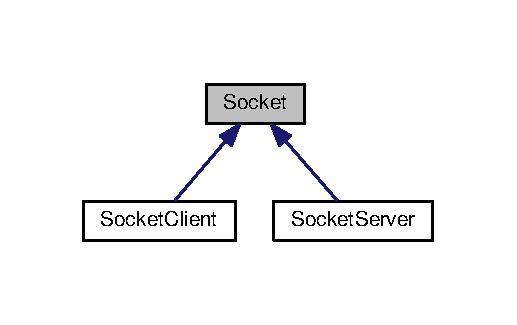
\includegraphics[width=248pt]{classSocket__inherit__graph}
\end{center}
\end{figure}
\subsection*{Public Member Functions}
\begin{DoxyCompactItemize}
\item 
\hyperlink{classSocket_a7c3256c4fc6e2c603df73201049fae5a}{Socket} ()
\begin{DoxyCompactList}\small\item\em Constructor of \hyperlink{classSocket}{Socket} Class. \end{DoxyCompactList}\item 
\hyperlink{classSocket_aeac4eb6379a543d38ed88977d3b6630a}{$\sim$\+Socket} ()
\begin{DoxyCompactList}\small\item\em Destructor of \hyperlink{classSocket}{Socket} Class. \end{DoxyCompactList}\item 
int \hyperlink{classSocket_ac4bde0cd12b53244b7c143d056b383ba}{get\+File\+Descriptor} ()
\begin{DoxyCompactList}\small\item\em Returns the file\+Descriptor held by the object. \end{DoxyCompactList}\end{DoxyCompactItemize}
\subsection*{Static Public Member Functions}
\begin{DoxyCompactItemize}
\item 
static bool \hyperlink{classSocket_a47696700f9178bb87ef800cb477ecacc}{get\+Ip\+From\+Name} (string hostname, struct hostent $\ast$\&host)
\begin{DoxyCompactList}\small\item\em Static function to fetch Ip address from domain\+Name/host\+Name. \end{DoxyCompactList}\item 
static bool \hyperlink{classSocket_a6b9394cf7656ec2f7ae86d57374379ca}{send\+\_\+data} (int file\+Descriptor, string data\+To\+Send)
\begin{DoxyCompactList}\small\item\em Send data to other end of socket. \end{DoxyCompactList}\item 
static int \hyperlink{classSocket_a76ba0cc2ab002c701fe8cbab31f95589}{recv\+\_\+data} (int file\+Descriptor, string \&recv\+Data\+Here)
\begin{DoxyCompactList}\small\item\em Recive data from other end of socket. \end{DoxyCompactList}\item 
static int \hyperlink{classSocket_a42c17ec1faed733a261a9160a45aa733}{close\+\_\+socket} (int file\+Descriptor)
\begin{DoxyCompactList}\small\item\em Close the \hyperlink{classSocket}{Socket}. \end{DoxyCompactList}\item 
static string \hyperlink{classSocket_a02ab07fcadca4429f50dcfebd7e63e9a}{get\+Name\+From\+FD} (int file\+Descriptor)
\begin{DoxyCompactList}\small\item\em Returns the IP address from File-\/descriptor. \end{DoxyCompactList}\end{DoxyCompactItemize}


\subsection{Detailed Description}
Class responsible for managin low-\/level sockets. 

This class encapsulates some low-\/level socket functionalities and provide an easy to use interface for handling the sockets. Some of the functions are static becuase they doesn\textquotesingle{}t require access to any class member and moreover need to be able to access these seperately. This function will put the response in the host or else will nullptr. 

\subsection{Constructor \& Destructor Documentation}
\index{Socket@{Socket}!Socket@{Socket}}
\index{Socket@{Socket}!Socket@{Socket}}
\subsubsection[{\texorpdfstring{Socket()}{Socket()}}]{\setlength{\rightskip}{0pt plus 5cm}Socket\+::\+Socket (
\begin{DoxyParamCaption}
{}
\end{DoxyParamCaption}
)}\hypertarget{classSocket_a7c3256c4fc6e2c603df73201049fae5a}{}\label{classSocket_a7c3256c4fc6e2c603df73201049fae5a}


Constructor of \hyperlink{classSocket}{Socket} Class. 

Creates/opens the low-\/level socket object. \index{Socket@{Socket}!````~Socket@{$\sim$\+Socket}}
\index{````~Socket@{$\sim$\+Socket}!Socket@{Socket}}
\subsubsection[{\texorpdfstring{$\sim$\+Socket()}{~Socket()}}]{\setlength{\rightskip}{0pt plus 5cm}Socket\+::$\sim$\+Socket (
\begin{DoxyParamCaption}
{}
\end{DoxyParamCaption}
)}\hypertarget{classSocket_aeac4eb6379a543d38ed88977d3b6630a}{}\label{classSocket_aeac4eb6379a543d38ed88977d3b6630a}


Destructor of \hyperlink{classSocket}{Socket} Class. 

Closes the low-\/level socket object. 

\subsection{Member Function Documentation}
\index{Socket@{Socket}!close\+\_\+socket@{close\+\_\+socket}}
\index{close\+\_\+socket@{close\+\_\+socket}!Socket@{Socket}}
\subsubsection[{\texorpdfstring{close\+\_\+socket(int file\+Descriptor)}{close_socket(int fileDescriptor)}}]{\setlength{\rightskip}{0pt plus 5cm}int Socket\+::close\+\_\+socket (
\begin{DoxyParamCaption}
\item[{int}]{file\+Descriptor}
\end{DoxyParamCaption}
)\hspace{0.3cm}{\ttfamily [static]}}\hypertarget{classSocket_a42c17ec1faed733a261a9160a45aa733}{}\label{classSocket_a42c17ec1faed733a261a9160a45aa733}


Close the \hyperlink{classSocket}{Socket}. 


\begin{DoxyParams}{Parameters}
{\em \textquotesingle{}int} & file\+Descriptor\textquotesingle{} \+: \hyperlink{classSocket}{Socket} which is to be closed. \\
\hline
\end{DoxyParams}
\begin{DoxyReturn}{Returns}
\textquotesingle{}int\textquotesingle{} \+: 0 on success, else -\/1. 
\end{DoxyReturn}
\index{Socket@{Socket}!get\+File\+Descriptor@{get\+File\+Descriptor}}
\index{get\+File\+Descriptor@{get\+File\+Descriptor}!Socket@{Socket}}
\subsubsection[{\texorpdfstring{get\+File\+Descriptor()}{getFileDescriptor()}}]{\setlength{\rightskip}{0pt plus 5cm}int Socket\+::get\+File\+Descriptor (
\begin{DoxyParamCaption}
{}
\end{DoxyParamCaption}
)}\hypertarget{classSocket_ac4bde0cd12b53244b7c143d056b383ba}{}\label{classSocket_ac4bde0cd12b53244b7c143d056b383ba}


Returns the file\+Descriptor held by the object. 

\begin{DoxyReturn}{Returns}
\textquotesingle{}int\textquotesingle{} \+: \hyperlink{classSocket}{Socket} File-\/\+Descriptor. 
\end{DoxyReturn}
\index{Socket@{Socket}!get\+Ip\+From\+Name@{get\+Ip\+From\+Name}}
\index{get\+Ip\+From\+Name@{get\+Ip\+From\+Name}!Socket@{Socket}}
\subsubsection[{\texorpdfstring{get\+Ip\+From\+Name(string hostname, struct hostent $\ast$\&host)}{getIpFromName(string hostname, struct hostent *&host)}}]{\setlength{\rightskip}{0pt plus 5cm}bool Socket\+::get\+Ip\+From\+Name (
\begin{DoxyParamCaption}
\item[{string}]{hostname, }
\item[{struct hostent $\ast$\&}]{host}
\end{DoxyParamCaption}
)\hspace{0.3cm}{\ttfamily [static]}}\hypertarget{classSocket_a47696700f9178bb87ef800cb477ecacc}{}\label{classSocket_a47696700f9178bb87ef800cb477ecacc}


Static function to fetch Ip address from domain\+Name/host\+Name. 

int m\+\_\+socket\+Fd \+: The socket file-\/descriptor associated with the object of this class

Fetch Ip from name and put in $\ast$host structure , passed via reference to the function. 
\begin{DoxyParams}{Parameters}
{\em \textquotesingle{}string} & hostname\textquotesingle{} \+: Hostname to fetch IP of. \\
\hline
{\em \textquotesingle{}struct} & hostent$\ast$ \&host\textquotesingle{} \+: To store the value of resolved IP address into this argument(passed via reference). \\
\hline
\end{DoxyParams}
\begin{DoxyReturn}{Returns}
\textquotesingle{}bool\textquotesingle{} \+: false if fails to resolve, else true. 
\end{DoxyReturn}
\index{Socket@{Socket}!get\+Name\+From\+FD@{get\+Name\+From\+FD}}
\index{get\+Name\+From\+FD@{get\+Name\+From\+FD}!Socket@{Socket}}
\subsubsection[{\texorpdfstring{get\+Name\+From\+F\+D(int file\+Descriptor)}{getNameFromFD(int fileDescriptor)}}]{\setlength{\rightskip}{0pt plus 5cm}string Socket\+::get\+Name\+From\+FD (
\begin{DoxyParamCaption}
\item[{int}]{file\+Descriptor}
\end{DoxyParamCaption}
)\hspace{0.3cm}{\ttfamily [static]}}\hypertarget{classSocket_a02ab07fcadca4429f50dcfebd7e63e9a}{}\label{classSocket_a02ab07fcadca4429f50dcfebd7e63e9a}


Returns the IP address from File-\/descriptor. 


\begin{DoxyParams}{Parameters}
{\em \textquotesingle{}int} & file\+Descriptor\textquotesingle{} \+: \hyperlink{classSocket}{Socket} which is to be closed. \\
\hline
\end{DoxyParams}
\begin{DoxyReturn}{Returns}
\textquotesingle{}string\textquotesingle{} \+: empty if fails to resolve, else IP address. 
\end{DoxyReturn}
\index{Socket@{Socket}!recv\+\_\+data@{recv\+\_\+data}}
\index{recv\+\_\+data@{recv\+\_\+data}!Socket@{Socket}}
\subsubsection[{\texorpdfstring{recv\+\_\+data(int file\+Descriptor, string \&recv\+Data\+Here)}{recv_data(int fileDescriptor, string &recvDataHere)}}]{\setlength{\rightskip}{0pt plus 5cm}int Socket\+::recv\+\_\+data (
\begin{DoxyParamCaption}
\item[{int}]{file\+Descriptor, }
\item[{string \&}]{recv\+Data\+Here}
\end{DoxyParamCaption}
)\hspace{0.3cm}{\ttfamily [static]}}\hypertarget{classSocket_a76ba0cc2ab002c701fe8cbab31f95589}{}\label{classSocket_a76ba0cc2ab002c701fe8cbab31f95589}


Recive data from other end of socket. 

Recieve the data and store it in the string argument which is passed by reference(\+M\+A\+N\+D\+A\+T\+O\+R\+Y). 
\begin{DoxyParams}{Parameters}
{\em \textquotesingle{}int} & file\+Descriptor\textquotesingle{} \+: \hyperlink{classSocket}{Socket} on which data is to be sent. \\
\hline
{\em \textquotesingle{}string} & \&recv\+Data\+Here\textquotesingle{} \+: Data which is to be recieved (pass by reference). \\
\hline
\end{DoxyParams}
\begin{DoxyReturn}{Returns}
\textquotesingle{}int\textquotesingle{} \+: Returns the size of data. 
\end{DoxyReturn}
\index{Socket@{Socket}!send\+\_\+data@{send\+\_\+data}}
\index{send\+\_\+data@{send\+\_\+data}!Socket@{Socket}}
\subsubsection[{\texorpdfstring{send\+\_\+data(int file\+Descriptor, string data\+To\+Send)}{send_data(int fileDescriptor, string dataToSend)}}]{\setlength{\rightskip}{0pt plus 5cm}bool Socket\+::send\+\_\+data (
\begin{DoxyParamCaption}
\item[{int}]{file\+Descriptor, }
\item[{string}]{data\+To\+Send}
\end{DoxyParamCaption}
)\hspace{0.3cm}{\ttfamily [static]}}\hypertarget{classSocket_a6b9394cf7656ec2f7ae86d57374379ca}{}\label{classSocket_a6b9394cf7656ec2f7ae86d57374379ca}


Send data to other end of socket. 


\begin{DoxyParams}{Parameters}
{\em \textquotesingle{}int} & file\+Descriptor\textquotesingle{} \+: \hyperlink{classSocket}{Socket} on which data is to be sent. \\
\hline
{\em \textquotesingle{}string} & data\+To\+Send\textquotesingle{} \+: Data which is to be sent. \\
\hline
\end{DoxyParams}
\begin{DoxyReturn}{Returns}
\textquotesingle{}bool\textquotesingle{} \+: false on failure to send, else true. 
\end{DoxyReturn}


The documentation for this class was generated from the following files\+:\begin{DoxyCompactItemize}
\item 
\hyperlink{Socket_8h}{Socket.\+h}\item 
Socket.\+cpp\end{DoxyCompactItemize}

\hypertarget{classSocketClient}{}\section{Socket\+Client Class Reference}
\label{classSocketClient}\index{Socket\+Client@{Socket\+Client}}


\textquotesingle{}\hyperlink{classSocketClient}{Socket\+Client}\textquotesingle{} inherits form \textquotesingle{}\hyperlink{classSocket}{Socket}\textquotesingle{} class and is specifically designed for client mode.  




{\ttfamily \#include $<$Socket\+Client.\+h$>$}



Inheritance diagram for Socket\+Client\+:
\nopagebreak
\begin{figure}[H]
\begin{center}
\leavevmode
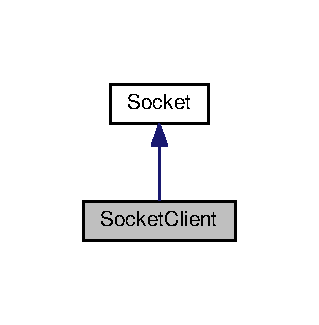
\includegraphics[width=153pt]{classSocketClient__inherit__graph}
\end{center}
\end{figure}


Collaboration diagram for Socket\+Client\+:
\nopagebreak
\begin{figure}[H]
\begin{center}
\leavevmode
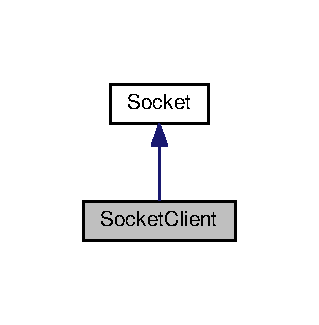
\includegraphics[width=153pt]{classSocketClient__coll__graph}
\end{center}
\end{figure}
\subsection*{Public Member Functions}
\begin{DoxyCompactItemize}
\item 
\hyperlink{classSocketClient_a80d1b7bfb8b4126d706981a80e05c78f}{Socket\+Client} ()\hypertarget{classSocketClient_a80d1b7bfb8b4126d706981a80e05c78f}{}\label{classSocketClient_a80d1b7bfb8b4126d706981a80e05c78f}

\begin{DoxyCompactList}\small\item\em Constructor of \hyperlink{classSocketClient}{Socket\+Client} Class. \end{DoxyCompactList}\item 
int \hyperlink{classSocketClient_ae2831125eccfceb142f9a9131677231a}{connect\+To\+Server} (string server\+Name, int port\+Number)
\begin{DoxyCompactList}\small\item\em Abstracted function to connects to the server. \end{DoxyCompactList}\end{DoxyCompactItemize}
\subsection*{Additional Inherited Members}


\subsection{Detailed Description}
\textquotesingle{}\hyperlink{classSocketClient}{Socket\+Client}\textquotesingle{} inherits form \textquotesingle{}\hyperlink{classSocket}{Socket}\textquotesingle{} class and is specifically designed for client mode. 

This class encapsulates some low-\/level client specific socket functionalities and provide an easy to use interface for handling the sockets. 

\subsection{Member Function Documentation}
\index{Socket\+Client@{Socket\+Client}!connect\+To\+Server@{connect\+To\+Server}}
\index{connect\+To\+Server@{connect\+To\+Server}!Socket\+Client@{Socket\+Client}}
\subsubsection[{\texorpdfstring{connect\+To\+Server(string server\+Name, int port\+Number)}{connectToServer(string serverName, int portNumber)}}]{\setlength{\rightskip}{0pt plus 5cm}int Socket\+Client\+::connect\+To\+Server (
\begin{DoxyParamCaption}
\item[{string}]{server\+Name, }
\item[{int}]{port\+Number}
\end{DoxyParamCaption}
)}\hypertarget{classSocketClient_ae2831125eccfceb142f9a9131677231a}{}\label{classSocketClient_ae2831125eccfceb142f9a9131677231a}


Abstracted function to connects to the server. 

Calls \textquotesingle{}socket\+\_\+connect\textquotesingle{} function which. 
\begin{DoxyParams}{Parameters}
{\em \textquotesingle{}string} & server\+Name \textquotesingle{} \+: Name of the server to connect to. \\
\hline
{\em \textquotesingle{}int} & port\+Number\textquotesingle{} \+: Port number of the server to connect on. \\
\hline
\end{DoxyParams}
\begin{DoxyReturn}{Returns}
\textquotesingle{}int\textquotesingle{} \+: returns what socket\+\_\+connect returns. 
\end{DoxyReturn}


The documentation for this class was generated from the following files\+:\begin{DoxyCompactItemize}
\item 
\hyperlink{SocketClient_8h}{Socket\+Client.\+h}\item 
Socket\+Client.\+cpp\end{DoxyCompactItemize}

\hypertarget{classSocketServer}{}\section{Socket\+Server Class Reference}
\label{classSocketServer}\index{Socket\+Server@{Socket\+Server}}


\textquotesingle{}\hyperlink{classSocketServer}{Socket\+Server}\textquotesingle{} inherits form \textquotesingle{}\hyperlink{classSocket}{Socket}\textquotesingle{} class and is specifically designed for server mode.  




{\ttfamily \#include $<$Socket\+Server.\+h$>$}



Inheritance diagram for Socket\+Server\+:
\nopagebreak
\begin{figure}[H]
\begin{center}
\leavevmode
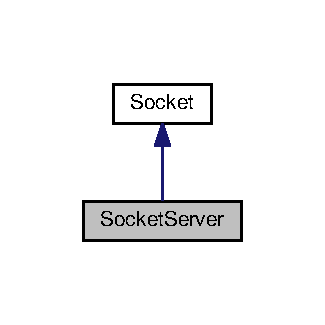
\includegraphics[width=156pt]{classSocketServer__inherit__graph}
\end{center}
\end{figure}


Collaboration diagram for Socket\+Server\+:
\nopagebreak
\begin{figure}[H]
\begin{center}
\leavevmode
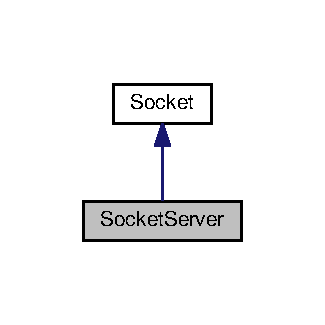
\includegraphics[width=156pt]{classSocketServer__coll__graph}
\end{center}
\end{figure}
\subsection*{Public Member Functions}
\begin{DoxyCompactItemize}
\item 
\hyperlink{classSocketServer_a262ba93dc8ad71b260fb75124b3453ee}{Socket\+Server} ()\hypertarget{classSocketServer_a262ba93dc8ad71b260fb75124b3453ee}{}\label{classSocketServer_a262ba93dc8ad71b260fb75124b3453ee}

\begin{DoxyCompactList}\small\item\em Constructor of \hyperlink{classSocketServer}{Socket\+Server} Class. \end{DoxyCompactList}\item 
int \hyperlink{classSocketServer_a50b619d415d32f52771b663b3036940c}{set\+Socket\+Options} ()
\begin{DoxyCompactList}\small\item\em Sets up the necessary socket options. \end{DoxyCompactList}\item 
int \hyperlink{classSocketServer_aaa25d38578f271ab252bf9f5ecafd2e4}{socket\+\_\+bind} (int port)
\begin{DoxyCompactList}\small\item\em Binds to the port on all interfaces. \end{DoxyCompactList}\item 
int \hyperlink{classSocketServer_af49cec86f9f7c45fbeca8b94c37ec0a1}{socket\+\_\+listen} ()
\begin{DoxyCompactList}\small\item\em Starts to listen for incoming connections on above set interfaces and port via file-\/descriptor(present in socket class). \end{DoxyCompactList}\item 
int \hyperlink{classSocketServer_add005b4dc2e06b847566952e52029585}{socket\+\_\+accept} ()
\begin{DoxyCompactList}\small\item\em Accepts the incoming socket connection.. \end{DoxyCompactList}\end{DoxyCompactItemize}
\subsection*{Static Public Member Functions}
\begin{DoxyCompactItemize}
\item 
static void \hyperlink{classSocketServer_a7e2e444c9cb9a1d146fe33536eee5b2e}{set\+\_\+nonblocking} (int file\+Descriptor)
\begin{DoxyCompactList}\small\item\em Sets the socket file-\/descriptor to non-\/blocking. \end{DoxyCompactList}\end{DoxyCompactItemize}


\subsection{Detailed Description}
\textquotesingle{}\hyperlink{classSocketServer}{Socket\+Server}\textquotesingle{} inherits form \textquotesingle{}\hyperlink{classSocket}{Socket}\textquotesingle{} class and is specifically designed for server mode. 

This class encapsulates some low-\/level server specific socket functionalities and provide an easy to use interface for handling the sockets. 

\subsection{Member Function Documentation}
\index{Socket\+Server@{Socket\+Server}!set\+\_\+nonblocking@{set\+\_\+nonblocking}}
\index{set\+\_\+nonblocking@{set\+\_\+nonblocking}!Socket\+Server@{Socket\+Server}}
\subsubsection[{\texorpdfstring{set\+\_\+nonblocking(int file\+Descriptor)}{set_nonblocking(int fileDescriptor)}}]{\setlength{\rightskip}{0pt plus 5cm}void Socket\+Server\+::set\+\_\+nonblocking (
\begin{DoxyParamCaption}
\item[{int}]{file\+Descriptor}
\end{DoxyParamCaption}
)\hspace{0.3cm}{\ttfamily [static]}}\hypertarget{classSocketServer_a7e2e444c9cb9a1d146fe33536eee5b2e}{}\label{classSocketServer_a7e2e444c9cb9a1d146fe33536eee5b2e}


Sets the socket file-\/descriptor to non-\/blocking. 

Sets the server FD to non-\/blocking, mandatorily required in order for server to be asynchronous. 
\begin{DoxyParams}{Parameters}
{\em \textquotesingle{}int} & file\+Descriptor\textquotesingle{} \+: \hyperlink{classSocket}{Socket} to set non-\/blocking on. \\
\hline
\end{DoxyParams}
\begin{DoxyReturn}{Returns}
void 
\end{DoxyReturn}
\index{Socket\+Server@{Socket\+Server}!set\+Socket\+Options@{set\+Socket\+Options}}
\index{set\+Socket\+Options@{set\+Socket\+Options}!Socket\+Server@{Socket\+Server}}
\subsubsection[{\texorpdfstring{set\+Socket\+Options()}{setSocketOptions()}}]{\setlength{\rightskip}{0pt plus 5cm}int Socket\+Server\+::set\+Socket\+Options (
\begin{DoxyParamCaption}
{}
\end{DoxyParamCaption}
)}\hypertarget{classSocketServer_a50b619d415d32f52771b663b3036940c}{}\label{classSocketServer_a50b619d415d32f52771b663b3036940c}


Sets up the necessary socket options. 

\begin{DoxyReturn}{Returns}
\textquotesingle{}int\textquotesingle{} \+: -\/1 if fails to setup , else 0. 
\end{DoxyReturn}
\index{Socket\+Server@{Socket\+Server}!socket\+\_\+accept@{socket\+\_\+accept}}
\index{socket\+\_\+accept@{socket\+\_\+accept}!Socket\+Server@{Socket\+Server}}
\subsubsection[{\texorpdfstring{socket\+\_\+accept()}{socket_accept()}}]{\setlength{\rightskip}{0pt plus 5cm}int Socket\+Server\+::socket\+\_\+accept (
\begin{DoxyParamCaption}
{}
\end{DoxyParamCaption}
)}\hypertarget{classSocketServer_add005b4dc2e06b847566952e52029585}{}\label{classSocketServer_add005b4dc2e06b847566952e52029585}


Accepts the incoming socket connection.. 

\begin{DoxyReturn}{Returns}
\textquotesingle{}int\textquotesingle{} \+: The file-\/\+Descriptor for accepted connection. 
\end{DoxyReturn}
\index{Socket\+Server@{Socket\+Server}!socket\+\_\+bind@{socket\+\_\+bind}}
\index{socket\+\_\+bind@{socket\+\_\+bind}!Socket\+Server@{Socket\+Server}}
\subsubsection[{\texorpdfstring{socket\+\_\+bind(int port)}{socket_bind(int port)}}]{\setlength{\rightskip}{0pt plus 5cm}int Socket\+Server\+::socket\+\_\+bind (
\begin{DoxyParamCaption}
\item[{int}]{port}
\end{DoxyParamCaption}
)}\hypertarget{classSocketServer_aaa25d38578f271ab252bf9f5ecafd2e4}{}\label{classSocketServer_aaa25d38578f271ab252bf9f5ecafd2e4}


Binds to the port on all interfaces. 


\begin{DoxyParams}{Parameters}
{\em \textquotesingle{}int} & port\textquotesingle{} \+: Port number for the server to bind on. \\
\hline
\end{DoxyParams}
\begin{DoxyReturn}{Returns}
\textquotesingle{}int\textquotesingle{} \+: -\/1 if fails to setup , else 0. 
\end{DoxyReturn}
\index{Socket\+Server@{Socket\+Server}!socket\+\_\+listen@{socket\+\_\+listen}}
\index{socket\+\_\+listen@{socket\+\_\+listen}!Socket\+Server@{Socket\+Server}}
\subsubsection[{\texorpdfstring{socket\+\_\+listen()}{socket_listen()}}]{\setlength{\rightskip}{0pt plus 5cm}int Socket\+Server\+::socket\+\_\+listen (
\begin{DoxyParamCaption}
{}
\end{DoxyParamCaption}
)}\hypertarget{classSocketServer_af49cec86f9f7c45fbeca8b94c37ec0a1}{}\label{classSocketServer_af49cec86f9f7c45fbeca8b94c37ec0a1}


Starts to listen for incoming connections on above set interfaces and port via file-\/descriptor(present in socket class). 

\begin{DoxyReturn}{Returns}
\textquotesingle{}int\textquotesingle{} \+: -\/1 if fails to setup , else 0. 
\end{DoxyReturn}


The documentation for this class was generated from the following files\+:\begin{DoxyCompactItemize}
\item 
\hyperlink{SocketServer_8h}{Socket\+Server.\+h}\item 
Socket\+Server.\+cpp\end{DoxyCompactItemize}

\chapter{File Documentation}
\hypertarget{Socket_8h}{}\section{Socket.\+h File Reference}
\label{Socket_8h}\index{Socket.\+h@{Socket.\+h}}


This file contains the \textquotesingle{}\hyperlink{classSocket}{Socket}\textquotesingle{} class.  


{\ttfamily \#include $<$netdb.\+h$>$}\\*
{\ttfamily \#include $<$arpa/inet.\+h$>$}\\*
{\ttfamily \#include $<$errno.\+h$>$}\\*
{\ttfamily \#include $<$fcntl.\+h$>$}\\*
{\ttfamily \#include $<$sys/socket.\+h$>$}\\*
{\ttfamily \#include $<$netinet/in.\+h$>$}\\*
Include dependency graph for Socket.\+h\+:
\nopagebreak
\begin{figure}[H]
\begin{center}
\leavevmode
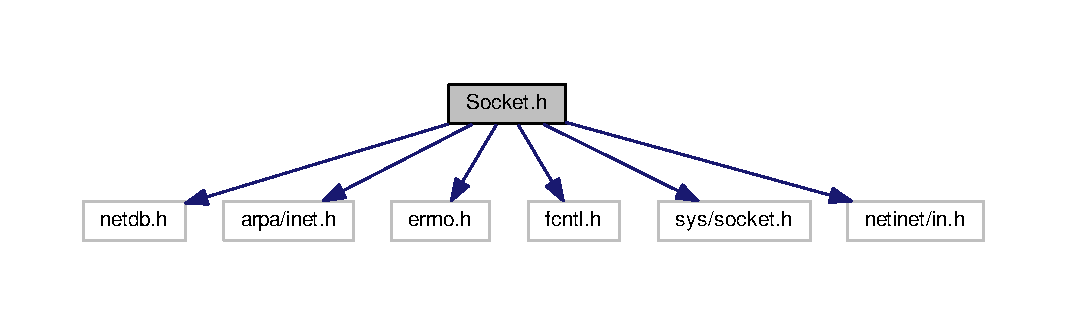
\includegraphics[width=350pt]{Socket_8h__incl}
\end{center}
\end{figure}
This graph shows which files directly or indirectly include this file\+:
\nopagebreak
\begin{figure}[H]
\begin{center}
\leavevmode
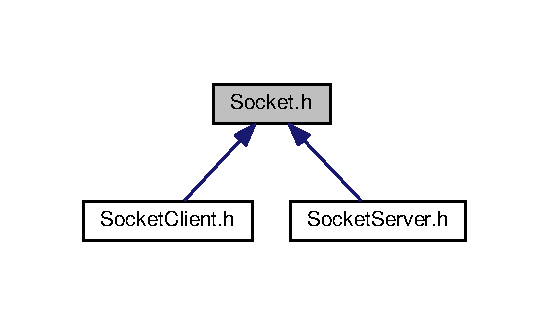
\includegraphics[width=264pt]{Socket_8h__dep__incl}
\end{center}
\end{figure}
\subsection*{Classes}
\begin{DoxyCompactItemize}
\item 
class \hyperlink{classSocket}{Socket}
\begin{DoxyCompactList}\small\item\em Class responsible for managin low-\/level sockets. \end{DoxyCompactList}\end{DoxyCompactItemize}
\subsection*{Macros}
\begin{DoxyCompactItemize}
\item 
\#define {\bfseries R\+E\+T\+U\+R\+N\+\_\+\+F\+A\+IL}~-\/1\hypertarget{Socket_8h_a837fc3a8b3b8209d20399ad2a02c1ae7}{}\label{Socket_8h_a837fc3a8b3b8209d20399ad2a02c1ae7}

\end{DoxyCompactItemize}


\subsection{Detailed Description}
This file contains the \textquotesingle{}\hyperlink{classSocket}{Socket}\textquotesingle{} class. 


\hypertarget{SocketClient_8h}{}\section{Socket\+Client.\+h File Reference}
\label{SocketClient_8h}\index{Socket\+Client.\+h@{Socket\+Client.\+h}}


This file contains the \textquotesingle{}\hyperlink{classSocketClient}{Socket\+Client}\textquotesingle{} class.  


{\ttfamily \#include \char`\"{}Socket.\+h\char`\"{}}\\*
Include dependency graph for Socket\+Client.\+h\+:
\nopagebreak
\begin{figure}[H]
\begin{center}
\leavevmode
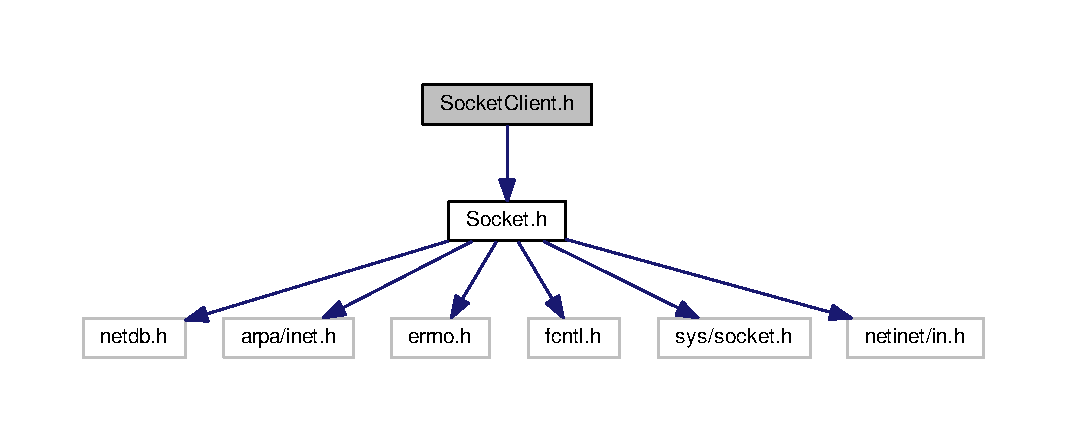
\includegraphics[width=350pt]{SocketClient_8h__incl}
\end{center}
\end{figure}
\subsection*{Classes}
\begin{DoxyCompactItemize}
\item 
class \hyperlink{classSocketClient}{Socket\+Client}
\begin{DoxyCompactList}\small\item\em \textquotesingle{}\hyperlink{classSocketClient}{Socket\+Client}\textquotesingle{} inherits form \textquotesingle{}\hyperlink{classSocket}{Socket}\textquotesingle{} class and is specifically designed for client mode. \end{DoxyCompactList}\end{DoxyCompactItemize}


\subsection{Detailed Description}
This file contains the \textquotesingle{}\hyperlink{classSocketClient}{Socket\+Client}\textquotesingle{} class. 


\hypertarget{SocketServer_8h}{}\section{Socket\+Server.\+h File Reference}
\label{SocketServer_8h}\index{Socket\+Server.\+h@{Socket\+Server.\+h}}


This file contains the \textquotesingle{}\hyperlink{classSocketServer}{Socket\+Server}\textquotesingle{} class.  


{\ttfamily \#include \char`\"{}Socket.\+h\char`\"{}}\\*
Include dependency graph for Socket\+Server.\+h\+:
\nopagebreak
\begin{figure}[H]
\begin{center}
\leavevmode
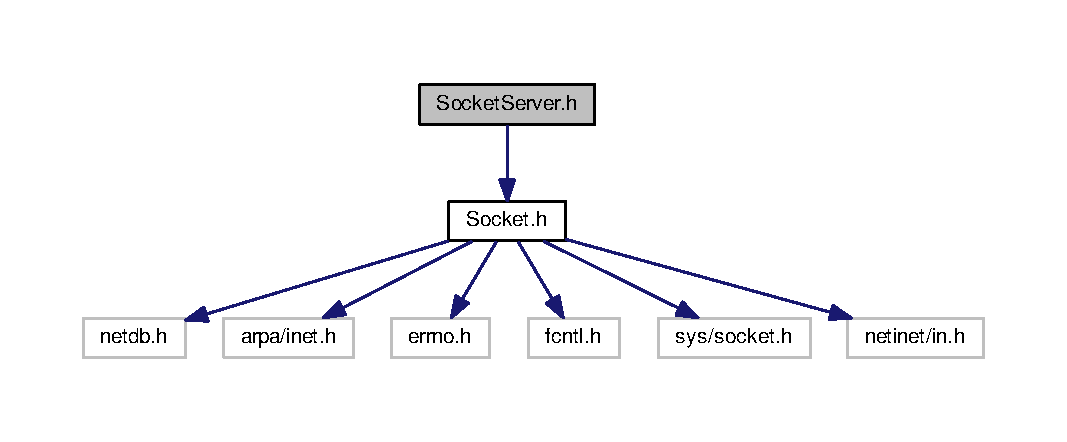
\includegraphics[width=350pt]{SocketServer_8h__incl}
\end{center}
\end{figure}
\subsection*{Classes}
\begin{DoxyCompactItemize}
\item 
class \hyperlink{classSocketServer}{Socket\+Server}
\begin{DoxyCompactList}\small\item\em \textquotesingle{}\hyperlink{classSocketServer}{Socket\+Server}\textquotesingle{} inherits form \textquotesingle{}\hyperlink{classSocket}{Socket}\textquotesingle{} class and is specifically designed for server mode. \end{DoxyCompactList}\end{DoxyCompactItemize}


\subsection{Detailed Description}
This file contains the \textquotesingle{}\hyperlink{classSocketServer}{Socket\+Server}\textquotesingle{} class. 


%--- End generated contents ---

% Index
\backmatter
\newpage
\phantomsection
\clearemptydoublepage
\addcontentsline{toc}{chapter}{Index}
\printindex

\end{document}
